% !TeX spellcheck = en_US
\addsection{New Elements}{\skills/pathfinding.png}

\begin{multicols*}{2}

\begin{center}
  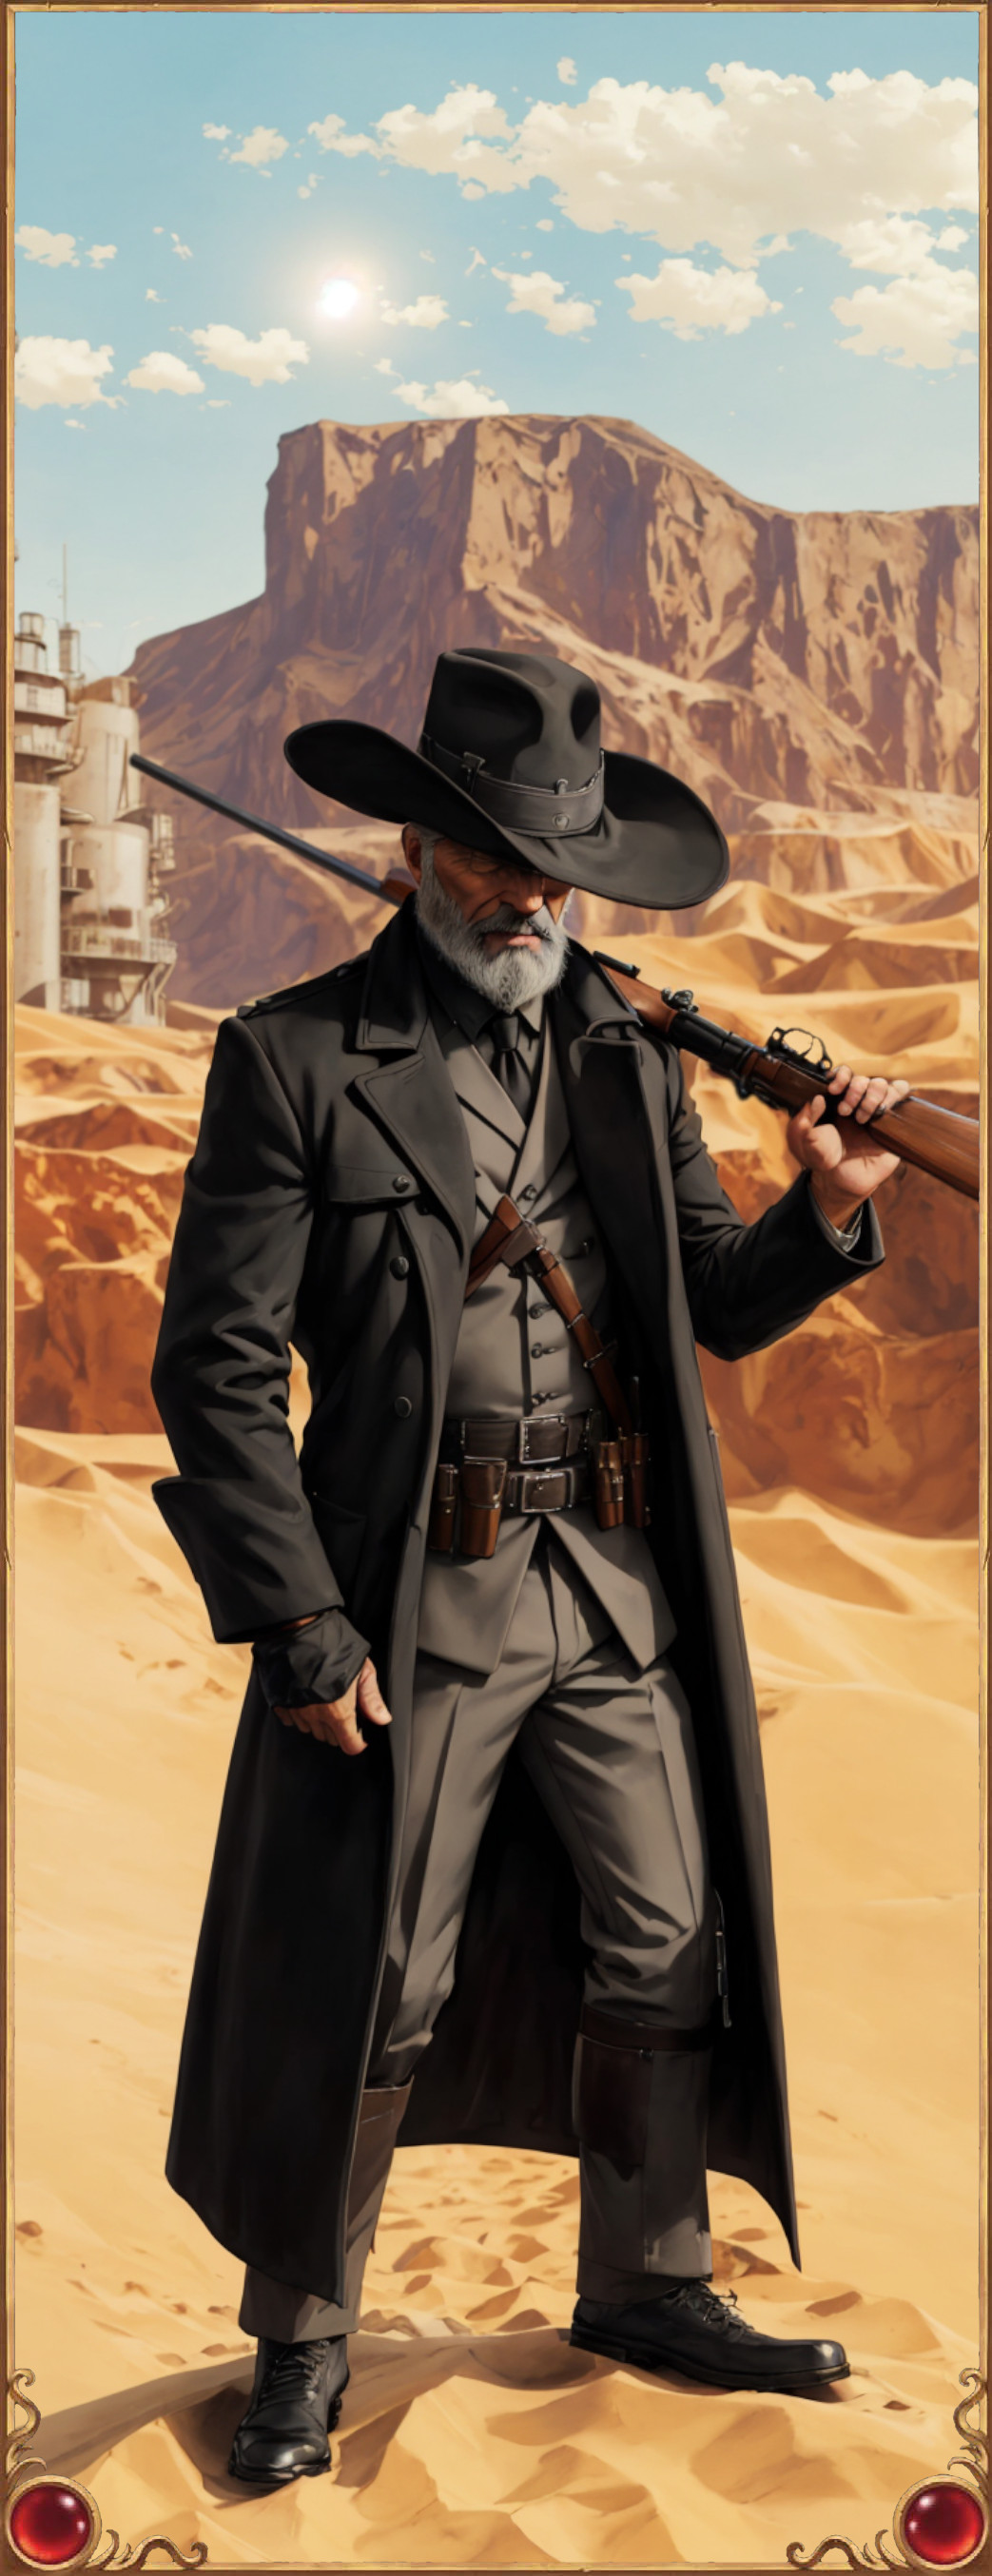
\includegraphics[width=\linewidth,height=\textheight,keepaspectratio]{\art/bounty_hunter.jpg}
\end{center}
\columnbreak

%\subsection*{\pagetarget{Quests}{Quests}}
\subheader{\pagetarget{Quests}{Quests}}

%Quests\index{Quests} are permanent Cards that can be bought at either a \pagelink{Trading Post}{Trading Post} or a \pagelink{War Machine Factory}{War Machine Factory}.
%If you buy one at the Trading Post, \textbf{you cannot use} any of the other normal functions of that Field during that Visit.
%War machines are also more expensive at the Trading Post.

The Factory expansion introduces “Quests\index{Quests} cards” \svg{quest_card}, which provide players with additional objectives to complete during the game.
Shuffle the Quest deck and place it face down near the game board.
Then, draw the top card and place it face up to create the discard pile.

{
  \bigskip
  \centering
  \begin{scriptsize}
    \begin{tikzpicture}
      \draw (0, 0) node[inner sep=0] {\makebox[\linewidth][c]{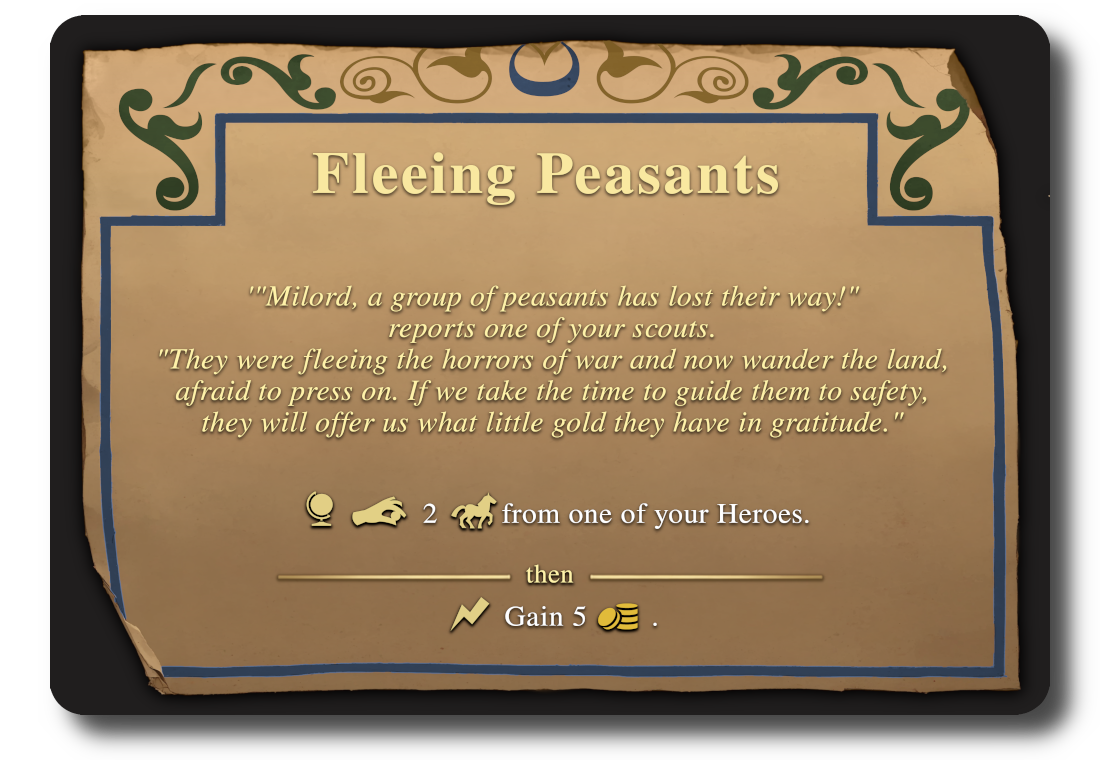
\includegraphics[width=\linewidth]{\cards/quest.png}}};
      \draw (0.4, 1.5) node {\encircle{\phantom{.}1\phantom{.}}};
      \draw (0, 0.2) node {\encircle{\phantom{.}2\phantom{.}}};
      \draw (-2.2, -0.95) node {\encircle{\phantom{.}3\phantom{.}}};
      \draw (-1.3, -1.7) node {\encircle{\phantom{.}4\phantom{.}}};
    \end{tikzpicture}
  \end{scriptsize}

  \footnotesize
  \textbf{\textit{\textcolor{darkcandyapplered}{Quest}}}

  \begin{multicols}{2}
    \begin{itemize}[itemsep=0pt, parsep=5pt, topsep=0pt, partopsep=0pt]
      \item[\textbf{1.}] Name
      \item[\textbf{2.}] Flavour text
      \item[\textbf{3.}] Requirement
      \item[\textbf{4.}] Reward
    \end{itemize}
  \end{multicols}
}

\subsection*{Structure of a Quest Card}

Each Quest card consists of two sections: Requirement and Reward.
There are two main types of Quests which differ significantly in the Requirement section:
\begin{itemize}
  \item \textbf{Non-Counter Quests} – These require a specific action to be performed (such as discarding cards or using abilities) or have a condition that must be met at a certain point in the game.
  The player may choose when to complete the Quest if the condition is met multiple times.
  \item \textbf{Counter Quests} – These require accumulating a certain number of \svg{quest_charge} tokens before they can be completed.
  When a player meets the condition to gain \svg{quest_charge}, they place a black cube on their Quest card.
  A Counter Quest can be completed at any time once it has at least the required number of \svg{quest_charge} tokens.
\end{itemize}

Once Quest is completed, the player immediately resolves the Reward effect and the card is removed from the game.

\subsection*{Acquiring and Managing Quests}
When a player gains a Quest, they place it face up next to their Hero or Town board.
A player may only have one active Quest at a time.
If a player gains a new Quest while already having an active one, they must discard the current Quest before accepting the new one.

Quests can be obtained from \pagelink{Seer’s Hut}{Seer’s Hut} locations, allowing a player to Search(2) Quests.
Seer’s Hut functions similarly to a Star Axis, meaning each player may use it only once.
Quests can also be acquired through new Astrologer effects and Event cards.
Just like other decks, Search(X) allows a player to take the top card from the discard pile.

By incorporating Quests into their strategy, players can gain powerful rewards that may turn the tide of the game.

{
  \bigskip
  \centering
  \begin{scriptsize}
    \begin{tikzpicture}
      \draw (0, 0) node[inner sep=0] {\makebox[0.47\linewidth][c]{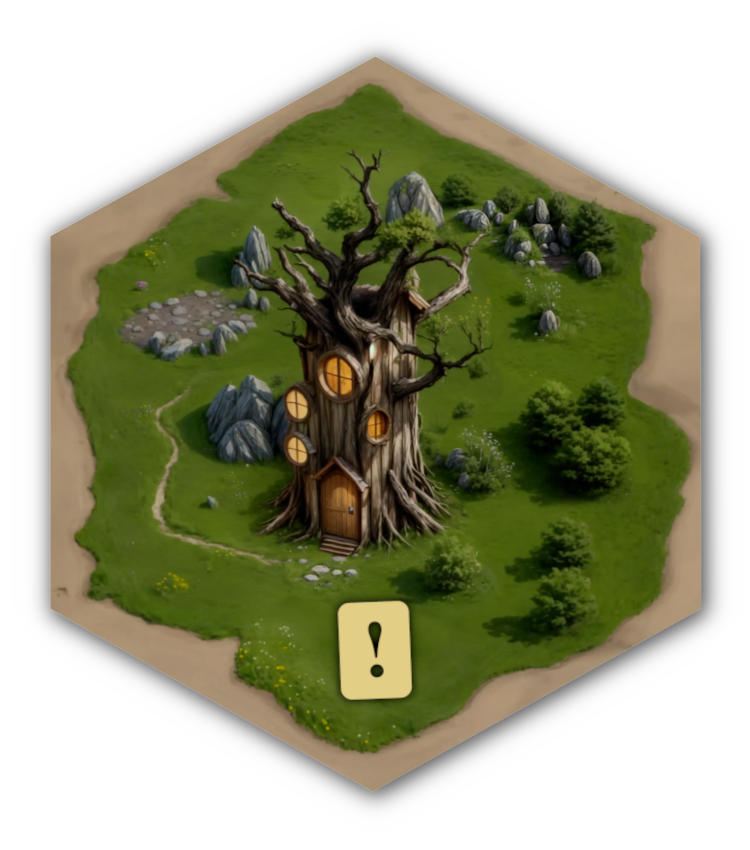
\includegraphics[width=0.47\linewidth]{\images/seers_hut.png}}};
    \end{tikzpicture}
  \end{scriptsize}

  \footnotesize
  \centering
  \textbf{\textit{\textcolor{darkcandyapplered}{Seer's Hut}}} \par
}

\vspace*{\fill}
\columnbreak


\subheader{\pagetarget{Map Locations}{Map Locations}}

In Factory Expansion, you will find more tiles with new locations to discover.
For the complete list of the locations, go to \pagelink{All Map Locations}{All Map Locations}.
% TODO: page link
\medskip

\subheader{\pagetarget{Mark Tokens}{Mark Tokens}}

\begin{tikzpicture}[overlay]
  \node at (7, 0) {
\includegraphics[width=0.2\linewidth]{\images/mark_token.png}};
\end{tikzpicture}\parbox{0.7\hsize}{Mark tokens are indicators placed on enemy units and are applied by units or abilities, enhancing strategic options during gameplay.}\par\smallskip
These tokens remain in play for the duration of the Combat and signify that the marked units are being targeted.
The specific effects of Mark tokens are detailed on the relevant cards, explaining how they influence the marked units.
Each unit can only have one Mark token applied to it.\par

\vfill
\hspace{2em}
\includegraphics[width=1.2\linewidth]{\art/implosion.png}
\vfill

\end{multicols*}
